\documentclass[11pt]{article}

\usepackage[margin=1in]{geometry}
\usepackage{amsmath,amssymb}
\usepackage{graphicx}
\usepackage{booktabs}
\usepackage[colorlinks=true,linkcolor=blue,citecolor=blue,urlcolor=blue]{hyperref}
\usepackage{natbib}

\graphicspath{{../figures/}}

% \code tokens (tags, filenames, test names) carry no discretionary
% breaks, so a paragraph containing one can have no acceptable line
% break at all.  emergencystretch gives TeX the slack to set those
% lines loose rather than overfull.
\setlength{\emergencystretch}{3em}

\newcommand{\rmu}{\ensuremath{\mathrm{rad\,m^{-2}}}}
\newcommand{\lamsq}{\ensuremath{\lambda^{2}}}
\newcommand{\code}[1]{\texttt{#1}}

\title{The diffuse Faraday signal as a delay-space template\\
  for LuSEE-Night: shape, bracket, and detectability}
\author{Christian Hellum Bye}
\date{2026-08-21}

\begin{document}
\maketitle

\begin{abstract}
\noindent
LuSEE-Night observes the polarized synchrotron sky through the Galactic
Faraday screen at 10--50\,MHz, where \lamsq{} is large enough that the
rotation measure distribution of the Galaxy is resolved in delay space.
This report derives the observable, states what can and cannot be
predicted from present inputs, and gives the detectability forecast.

The central result is methodological and it reverses a previous
conclusion. Summing the Faraday phasor pixel by pixel over a HEALPix map
is a random walk whose amplitude falls as $N_{\rm pix}^{-1/2}$: at
nside 512 the earlier diffuse calculation was measuring pixelisation
shot noise rather than sky. Binning the beam- and emissivity-weighted
sky \emph{in Faraday depth first} and transforming second gives a
distribution $F(\phi)$ whose \emph{shape} is invariant under refinement,
with the shot noise confined to the normalisation. The shape is
therefore predictable; the amplitude is not, and is quoted as a bracket
with reasons rather than as a value.

Of the three bands, 30\,MHz is the one where Faraday resolution
($7.59$\,\rmu{} amplitude FWHM) and depth reach ($604$\,\rmu{} zoom
horizon) line up, and it hosts the template's 90\%-mass knee at
$89.6$\,\rmu. 50\,MHz has the coarsest resolution but is the only band
whose horizon clears the map maximum; 10\,MHz has the sharpest
resolution and nothing within reach to resolve.

Against a $5\sigma$ whitened matched filter on the true zoom-bin
covariance at 24 lunations, the Galactic-Centre-transit tail exceeds
threshold by $4.7\times$ at 30\,MHz and $19.3\times$ at 50\,MHz if the
diffuse amplitude sits at the uniform-slab depolarisation floor, and
falls below threshold at every band if it sits at the internal-dispersion
floor. The gate is therefore decided by which depolarisation floor the
interstellar medium sets --- a mixed-versus-external-screen geometry
question --- and not by the tail measurement, not by the coherence angle,
and not by integration time: closing the 30\,MHz gap by integrating
alone would take $\sim\!3\times10^{4}$ times more nights.
\end{abstract}

\tableofcontents

\section{Scope, and what this supersedes}
\label{sec:scope}

\subsection{What is predicted, and what is not}

This report predicts a \emph{normalised shape} in Faraday depth and a
detectability threshold against it. It does not predict the amplitude of
the diffuse Faraday signal. That split is not a hedge; it follows from
what the inputs can support, and Section~\ref{sec:cannot} shows exactly
where the amplitude calculation runs out of information.

Three things are inputs, not results, and are owned elsewhere:
the instrument response and the covariance assembly (\code{luseepy}),
the spherical transforms and the polarized harmonic dual
(\code{croissant}), and the Galactic Faraday depth map
\citep{hutschenreuter2022}. This work owns the layer above: how a
Faraday-rotated sky enters that formalism, and how the result is read out
in delay space.

\subsection{Relation to the earlier analysis}
\label{sec:supersede}

An earlier four-port analysis of the same instrument, together with the
numerical audit that refuted part of it, is preserved at the repository
tag \code{audit-2026-08-18}. The status of that document, section by
section:

\begin{center}
\begin{tabular}{lll}
\toprule
Earlier section & Status & Where it now lives \\
\midrule
Step 0, calibrated polarimeter & stands & unchanged \\
Step 1, single polarized source & stands & regenerated, $\le0.6\%$ moves \\
Step 3, 10 and 50\,MHz bands & stands & unchanged \\
Perfect-depolarisation ($I$-only) limit & stands & unchanged \\
\midrule
Step 2, the real sky at 30\,MHz & \textbf{refuted} & this report, \S\ref{sec:randomwalk}--\ref{sec:depthdist} \\
Step 4, delay-space signature & \textbf{refuted} & this report, \S\ref{sec:depthdist}--\ref{sec:verdict} \\
\bottomrule
\end{tabular}
\end{center}

The refutation is specific and is reproduced with its mathematics in
Section~\ref{sec:randomwalk}: the diffuse Faraday signature reported in
those two sections was a HEALPix pixelisation artifact. The quantity
$|\Delta P|/I \sim 1.7\times10^{-4}$ that appeared there, and the Step-4
amplitude, do not appear here in any form. Cite the tag, not a branch,
when referring to the refuted results.

Nothing in this report modifies that document. It is a standalone
treatment of the delay-space template, and Section~\ref{sec:repro} lists
the code, data products and tests that produce every number in it.

\section{Faraday rotation in the harmonic dual}
\label{sec:dual}

\subsection{The rotation}

For a linearly polarized sky described by Stokes $Q,U$, propagation
through a magnetised plasma of Faraday depth $\phi$ rotates the
polarization vector. In the \code{healpy}/COSMO convention used for all
input maps,
\begin{equation}
  (Q + iU)_{\rm COSMO} \;\longrightarrow\; (Q + iU)_{\rm COSMO}\,
  e^{+2i\phi\lamsq},
  \label{eq:faraday}
\end{equation}
with $\lamsq = (c/\nu)^2$ in $\mathrm{m^2}$ and $\phi$ in \rmu. The
factor of two is the spin weight of linear polarization: a rotation of
the plane of polarization by $\chi = \phi\lamsq$ advances $Q+iU$ by
$2\chi$.

Two convention conversions have to travel with
Equation~\eqref{eq:faraday} or signs are lost. Spherical-harmonic
machinery consumes the IAU convention, in which $U_{\rm IAU} = -U_{\rm
COSMO}$, so for real maps
\begin{equation}
  (Q+iU)_{\rm IAU} = \overline{(Q+iU)_{\rm COSMO}} .
\end{equation}

\subsection{Why the frequency axis is free}

The polarized harmonic dual holds two spin-$\pm2$ blocks: $P_{-}$, the
spin $-2$ analysis of $(Q+iU)_{\rm IAU}$, and $P_{+}$, the spin $+2$
analysis of $(Q-iU)_{\rm IAU}$, alongside the spin-0 blocks $I$ and $V$.
Combining the two conversions above, Faraday rotation acts on the dual as
\begin{equation}
  \bigl(I,\;V,\;P_{-},\;P_{+}\bigr) \;\longrightarrow\;
  \bigl(I,\;V,\;e^{-2i\phi\lamsq}P_{-},\;e^{+2i\phi\lamsq}P_{+}\bigr).
  \label{eq:dualblock}
\end{equation}

Equation~\eqref{eq:dualblock} is the structural fact the whole
calculation rests on: \textbf{Faraday rotation is diagonal in the
harmonic dual}. It multiplies each block by a scalar that depends on
frequency and on the depth $\phi$, but not on $\ell$ or $m$. A region of
constant Faraday depth therefore needs one frequency-independent set of
$a_{\ell m}$ plus a per-frequency, per-block scalar coefficient.

The consequence is computational and it is what makes the 16\,384-channel
fine grid affordable. The expensive object --- the contraction of sky
harmonics against instrument-response harmonics --- is computed once per
sky component, and the frequency dependence is applied afterwards as a
multiplication by scalars. Without Equation~\eqref{eq:dualblock} the
contraction would have to be repeated per channel.

\section{The four-port response and the Faraday weight}
\label{sec:weight}

The instrument is a four-port monopole--dipole antenna system, ports
labelled $\mathrm{N,E,S,W} = 0,1,2,3$, read out as sixteen real
cross-power channels. For each port pair the response to the sky is
expressed as a pair-Stokes kernel $\bigl(K_I, K_Q, K_U, K_V\bigr)(\hat n)$:
the sensitivity of that pair's cross power to each Stokes parameter
arriving from direction $\hat n$.

A Faraday-rotated sky enters through $K_Q$ and $K_U$ only. Under
Equation~\eqref{eq:faraday} the linear-polarization response of a pair to
a direction of depth $\phi$ is
\begin{equation}
  K_Q\,Q + K_U\,U \;=\;
  \Re\Bigl[\bigl(K_Q - iK_U\bigr)\,(Q+iU)\,e^{2i\phi\lamsq}\Bigr],
\end{equation}
so the modulus of the complex kernel $K_Q - iK_U$ sets how strongly that
direction contributes to the Faraday signal. Because the intrinsic
polarization angle of the sky is unknown and effectively random from
direction to direction, the quantity that survives is the
\emph{basis-independent} combination
\begin{equation}
  \bigl|w(\hat n)\bigr| \;=\;
  \sqrt{\tfrac12\Bigl(\bigl|K_Q(\hat n)\bigr|^2 + \bigl|K_U(\hat
  n)\bigr|^2\Bigr)},
  \label{eq:weight}
\end{equation}
averaged over port pairs and over local sidereal time.
Equation~\eqref{eq:weight} combines \emph{both} Faraday branches; using
$|K_Q|$ alone would make the weight --- and therefore every percentile
and every template below --- depend on the arbitrary orientation of the
$Q$/$U$ basis.

Figure~\ref{fig:weight} is $|w|^2$ for the as-built four-port response.
Two features matter downstream. The Galactic plane dominates, which is
why the plane taper of Section~\ref{sec:robust} moves the roll-off so
far. And $4.2\%$ of the sky --- a contiguous cap around
$l \approx 70^\circ\!-\!125^\circ$, $b \approx 5^\circ\!-\!53^\circ$ ---
carries exactly zero weight: it never rises above the horizon at the
landing site over the sidereal cycle, and contributes to no template at
any band.

\begin{figure}[htbp]
  \centering
  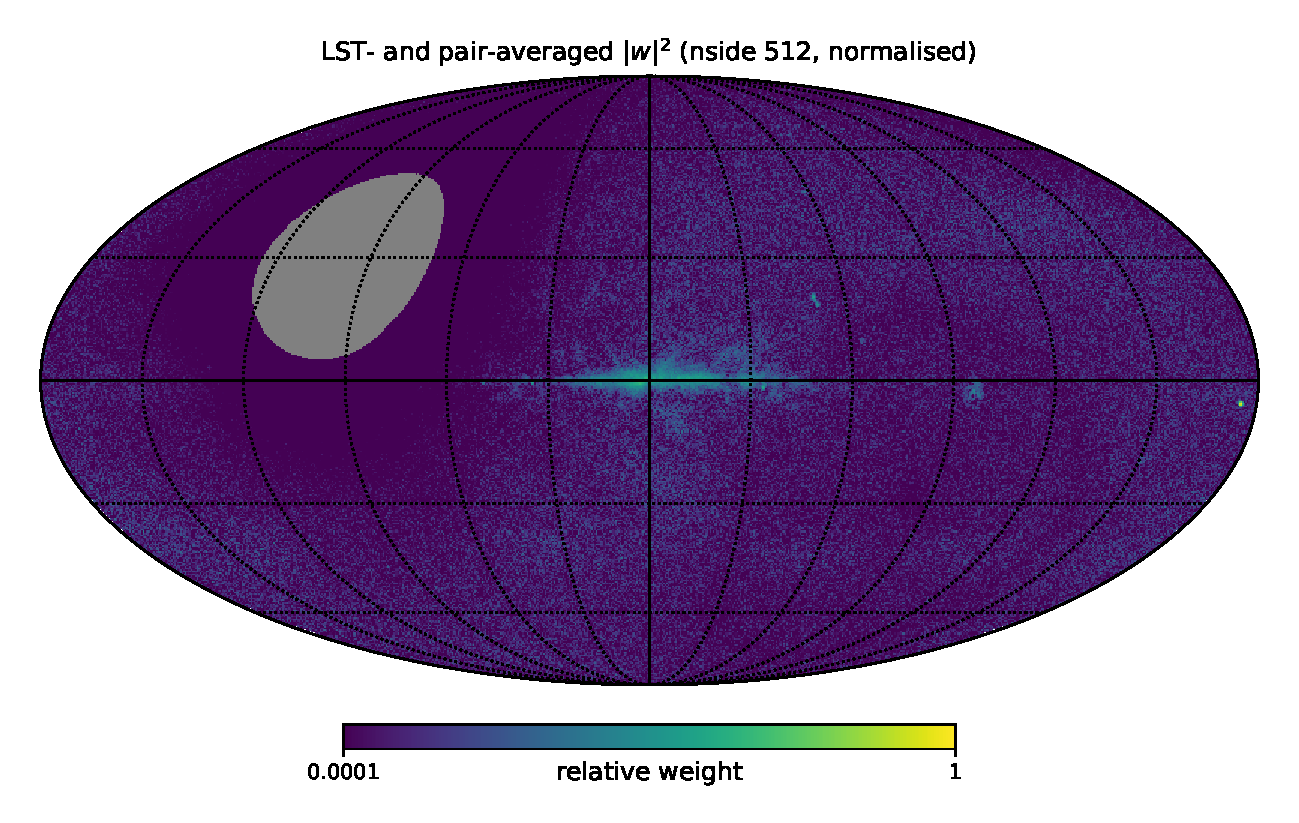
\includegraphics[width=0.72\textwidth]{step5_weight_map.pdf}
  \caption{The LST- and pair-averaged Faraday weight $|w|^2$ of the
  as-built four-port response, Equation~\eqref{eq:weight}, at
  nside 512 in Galactic coordinates, normalised to its peak and shown on
  a logarithmic scale clipped at $10^{-4}$. Grey: the $4.2\%$ of sky
  never above the horizon, which carries exactly zero weight. Every sky
  percentile quoted in this report is weighted by this map.}
  \label{fig:weight}
\end{figure}

Because the beam enters the diffuse calculation \emph{only} through
$|w(\hat n)|^2$, swapping the as-built four-port response for the
symmetric two-port pseudo-dipole is a single input substitution. That
makes the arm comparison in Section~\ref{sec:robust} a genuine
robustness test rather than a re-derivation.

\section{Why the pixel-space sum fails}
\label{sec:randomwalk}

The earlier calculation formed the observable as a coherent sum over
HEALPix pixels,
\begin{equation}
  P(\lamsq) \;=\; \sum_{n} w_n\, e^{2i\phi_n \lamsq},
  \label{eq:pixelsum}
\end{equation}
with $\phi_n$ the Faraday depth of pixel $n$ and $w_n$ its complex
weight, and read an amplitude off the result. That estimator does not
converge to a sky quantity.

Write $w_n = |w_n| e^{i\alpha_n}$ and $\theta_n = \alpha_n +
2\phi_n\lamsq$. The intrinsic polarization angles $\alpha_n$ are
effectively random between pixels, and so is $2\phi_n\lamsq$ modulo
$2\pi$: at nside 512 the Faraday depth changes by of order
$10^{3}$\,\rmu{} between neighbouring pixels, so at 30\,MHz
($\lamsq = 99.86\,\mathrm{m^2}$) the phase advances by hundreds of turns
from one pixel to the next. Then
\begin{equation}
  \bigl\langle |P|^2 \bigr\rangle
  = \sum_{n,m} |w_n||w_m| \bigl\langle e^{i(\theta_n - \theta_m)}
  \bigr\rangle
  = \sum_{n} |w_n|^2 ,
  \label{eq:walk}
\end{equation}
because every cross term averages to zero. For $N$ pixels of comparable
weight $|w|$ this gives $\langle|P|^2\rangle = N|w|^2$, and the
\emph{normalised} amplitude behaves as
\begin{equation}
  \frac{\sqrt{\langle |P|^2\rangle}}{\sum_n |w_n|}
  \;=\; \frac{\sqrt{N}\,|w|}{N|w|}
  \;=\; N^{-1/2}.
  \label{eq:nhalf}
\end{equation}

Equation~\eqref{eq:nhalf} is a statement about the \emph{estimator}, not
about the sky. Its value is set by how finely the sphere happens to be
pixelised, and it has no limit as the pixelisation is refined: it goes to
zero. Figure~\ref{fig:chirp} is not this test; the direct demonstration
is the acceptance gate of Section~\ref{sec:gates}, where refining
nside 256 $\rightarrow$ 2048 collapses the coherent power from
$8.42\times10^{-7}$ to $6.26\times10^{-9}$ --- a factor $134$ over a
$64\times$ refinement, close to the factor $64$ that
Equation~\eqref{eq:nhalf} predicts and nothing like the invariance a
physical signal would show.

The failure is not a bug in the implementation of
Equation~\eqref{eq:pixelsum}; the sum is computed correctly. It is that
the coherent pixel sum is the wrong estimator for a quantity whose phases
decorrelate below the pixel scale.

\section{The depth distribution and its transform}
\label{sec:depthdist}

\subsection{Bin first, transform second}

Reverse the order of operations. Define the beam- and
emissivity-weighted \emph{Faraday depth distribution}
\begin{equation}
  F(\phi)\,\mathrm d\phi \;=\;
  \text{weight arriving from depths in } [\phi, \phi + \mathrm d\phi],
\end{equation}
built by accumulating $|w_n|^2$ into depth bins, and take the transform
afterwards:
\begin{equation}
  P(\lamsq) \;=\; \int F(\phi)\, e^{2i\phi\lamsq}\,\mathrm d\phi .
  \label{eq:rmsynth}
\end{equation}
Equation~\eqref{eq:rmsynth} is the standard RM-synthesis relation
\citep{burn1966,brentjens2005}. What changes is not the physics but the
order: binning is a histogram operation, and a histogram's \emph{shape}
is stable under refinement of the sphere because refining splits each
pixel's weight among sub-pixels of nearly the same depth. The shot noise
of Equation~\eqref{eq:nhalf} has not disappeared --- it is confined to
the normalisation, which is precisely the quantity this report declines to
predict.

Both directions of Equation~\eqref{eq:rmsynth} are evaluated as type-3
nonuniform FFTs \citep{barnett2019} on the \emph{true} \lamsq{} nodes.
This is not an optimisation; see Section~\ref{sec:chirp}.

\subsection{The emissivity geometry: the $f^k$ pushforward}
\label{sec:pushforward}

$F(\phi)$ is not the histogram of the Faraday depth map. The map gives
$\phi_{{\rm col},n}$, the depth of the \emph{entire} column along
sightline $n$. Emission originating partway along that column is rotated
only by the fraction of the column in front of it.

Parameterise position along the column by $f\in[0,1]$, with $f=0$ at the
observer and $f=1$ at the far end, and let the synchrotron emissivity
vary as
\begin{equation}
  \rho(f) \;\propto\; f^{k}, \qquad k \ge -1 .
\end{equation}
Emission from $f$ accumulates depth $\phi = f\,\phi_{\rm col}$. The
cumulative distribution of depth contributed by sightline $n$ is then
\begin{align}
  \mathrm{CDF}_n(e)
  &= \Pr\bigl[f\,\phi_{{\rm col},n} \le e\bigr]
   = \Pr\bigl[f \le e/\phi_{{\rm col},n}\bigr] \nonumber\\[2pt]
  &= \frac{\displaystyle\int_0^{\min(e/\phi_{{\rm col},n},\,1)} f^{k}\,
     \mathrm df}{\displaystyle\int_0^{1} f^{k}\,\mathrm df}
   = \min\!\left(\frac{e}{\phi_{{\rm col},n}},\,1\right)^{\,k+1}.
  \label{eq:pushforward}
\end{align}
The distribution $F$ is the $|w_n|^2$-weighted sum of
Equation~\eqref{eq:pushforward} over sightlines, differenced onto depth
bins. The condition $k \ge -1$ is exactly the integrability of $f^k$ at
the origin; for $k < -1$ the normalising integral diverges and no
distribution exists.

Three values of $k$ bracket the geometry, and all three appear in the
template family:
\begin{itemize}
  \item $k \to \infty$: all emission at the far end,
    $F$ is the $|w|^2$-weighted histogram of $\phi_{\rm col}$ itself;
  \item $k = 0$: uniform slab, $\mathrm{CDF}_n(e) = \min(e/\phi_{\rm
    col},1)$, i.e. $F$ is a superposition of top-hats on
    $[0,\phi_{{\rm col},n}]$ --- \textbf{the fiducial};
  \item $k \to -1$: all emission local, $F \to \delta(\phi)$.
\end{itemize}

Every finite-$k$ pushforward places mass at $\phi = 0$, because every
column has a near end. The depth grid must therefore bracket zero; an
all-positive grid silently misplaces that mass, and the implementation
raises rather than returning a wrong histogram.

\subsection{The incoherent limit, and what it does and does not show}
\label{sec:identity}

The load-bearing claim connecting $F$ to the observable is that in the
incoherent limit the \emph{delay power} of the measured spectrum equals
the $|w|^2$-weighted depth distribution. Substituting
Equation~\eqref{eq:pixelsum} into the delay transform and expanding,
\begin{equation}
  \bigl\langle |\tilde P(\phi)|^2 \bigr\rangle
  \;=\; \sum_{n} |w_n|^2 \,\bigl|R(\phi - \phi_n)\bigr|^2
  \;+\; \underbrace{\sum_{n \ne m} |w_n||w_m|\,
    \bigl\langle e^{i(\alpha_n - \alpha_m)}\bigr\rangle\,
    R(\phi-\phi_n) \overline{R(\phi-\phi_m)}}_{\to\,0},
  \label{eq:identity}
\end{equation}
where $R$ is the point-spread function of Section~\ref{sec:rmsf}. The
first term \emph{is} $F$ convolved with $|R|^2$. So the same coherent sum
that fails as an \emph{amplitude} estimator succeeds as a
\emph{delay-power} estimator --- the shot noise of
Equation~\eqref{eq:walk} is exactly the diagonal term that
Equation~\eqref{eq:identity} wants.

Measured directly, with the real WMAP K-band polarization angles
\citep{bennett2013} supplying the pixel phases $\alpha_n$, the ratio of
the two sides is
\begin{equation}
  \frac{\text{delay power of the coherent pixel sum}}{|w|^2\text{-weighted
  depth distribution}} \;=\; 1.069
  \quad (30 \le |\phi| < 1500\,\rmu,\ 30\,\text{MHz}),
\end{equation}
and $1.332$ integrated over the whole axis. The difference between the
two is the $|\phi| < 10$ region, where the pixel sum is genuinely partly
coherent and the ratio alone is $1.92$.

\paragraph{How to read 1.069.} As an \emph{independent confirmation that
the ratio is consistent with unity}, not as a reproduction of a
particular number. The earlier audit's comparable figure, $1.038$, is a
different statistic --- different window, grid and estimator, and
unrestricted in range --- and is itself one of a series running
$1.010 / 1.184 / 1.038 / 0.843$ across nside, carrying $\sim13\%$
scatter. What the measurement adds is that a second estimator built from
different machinery lands in the same place.

\paragraph{That it is a test, not an identity.} Falsification probes
break it: building the model with $k=0$ against a $k\to\infty$
observable gives $1.85$, a shuffled RM map gives $1.58$, and the
$\mathrm{RM}\times0.02$ converged control --- where the depth
distribution collapses inside one resolution element --- fails by more
than $10^4$.

\paragraph{Two limits on what it shows.} It does \emph{not} demonstrate
that the sky is incoherent. Setting $\alpha_n \equiv 0$, every pixel
phase identical and maximally coherent, still passes at $0.889$. The
reason is in Equation~\eqref{eq:identity}: one turn of the
$e^{2i\phi\lamsq}$ carrier is a depth separation of only
$\pi/\lamsq = 0.0315$\,\rmu{} at 30\,MHz, so two pixels one resolution
element apart ($6.29$\,\rmu) are $\sim\!200$ turns apart and the cross
terms cancel by oscillation rather than by phase randomness. That makes
the identity \emph{more} robust than ``the sky happens to be
incoherent'' --- but it is not evidence of it. Nor does it pass only
because WMAP K per-pixel noise randomises the angles: smoothing $Q$ and
$U$ to $3^\circ$ and $10^\circ$ gives $1.107$ and $1.143$.

\subsection{The acceptance gates}
\label{sec:gates}

Two claims, two tests, and they must not be conflated.

\emph{The model's shape is pixelisation-stable.} The normalised
$F(\phi)$ moves by Kolmogorov distances of $2\times10^{-5}$ to
$1.9\times10^{-4}$ across nside 256--2048 and under a rigid null
rotation of the map, against a $10^{-2}$ tolerance, while the coherent
observable of Equation~\eqref{eq:pixelsum} collapses by $134\times$
under the same refinement and moves by $7.2\times$ under the rotation
alone.

\emph{These gates do not test the identity of
Section~\ref{sec:identity}.} With the uniform weights they use, a rigid
rotation is a pixel permutation that leaves the statistic invariant by
construction, and the nside 1024 and 2048 legs are interpolated
upsamplings of the native 512 map carrying no new sky. The identity is
covered by the direct measurement above, and by nothing else here.

\section{Resolution, envelope, and horizon}
\label{sec:resolution}

\subsection{The point-spread function in Faraday depth}
\label{sec:rmsf}

The instrument samples \lamsq{} at the centres of its spectrometer bins.
For the zoom mode this is 192 bins spaced $390.625$\,Hz apart, spanning
$\Delta\nu = 74\,609$\,Hz --- \emph{not} the fine grid's
$199\,988$\,Hz, which is the span that would apply if every fine channel
were an independent sample. The response to a unit Faraday tone is
\begin{equation}
  R(\phi) \;=\; \frac{1}{\Delta\lamsq}
  \int e^{2i\phi(\lamsq - \lamsq_0)}\, \mathrm d\lamsq
  \;=\; \operatorname{sinc}\!\bigl(\phi\,\Delta\lamsq\bigr),
  \qquad \operatorname{sinc}x = \frac{\sin x}{x},
  \label{eq:rmsfideal}
\end{equation}
for ideal top-hat coverage of a \lamsq{} span $\Delta\lamsq$. The
implementation does not assume Equation~\eqref{eq:rmsfideal}: it carries
a unit tone through the \emph{true} bin weight matrix and transforms over
the bin centres, so the measured $R$ includes the real bin shapes.

\paragraph{Two conventions, or the number is meaningless.} The
implementation returns \emph{power}, so a width read straight off it is a
power FWHM. The conventional RM-synthesis resolution is an
\emph{amplitude} FWHM. For the sinc of Equation~\eqref{eq:rmsfideal},
$|\operatorname{sinc}x| = 1/\sqrt2$ at $x = 1.3916$ and
$|\operatorname{sinc}x| = 1/2$ at $x = 1.8955$, so
\begin{equation}
  \frac{\text{power FWHM}}{\text{amplitude FWHM}}
  = \frac{1.3916}{1.8955} = 0.734 ,
  \qquad
  \text{amplitude FWHM}_{\rm ideal} = \frac{2 \times 1.8955}{\Delta\lamsq}.
  \label{eq:conventions}
\end{equation}

\begin{table}[htbp]
  \centering
  \caption{Faraday resolution from the true zoom-bin responses,
  measured by interpolated half-maximum crossings on an 80\,001-point
  $\phi$ grid. Both FWHM columns are measured independently rather than
  related by Equation~\eqref{eq:conventions}. Units \rmu.}
  \label{tab:rmsf}
  \begin{tabular}{lccc}
    \toprule
    Band & power FWHM & \textbf{amplitude FWHM} & ideal top-hat, same span \\
    \midrule
    30\,MHz & 5.574  & \textbf{7.592}  & 7.632 \\
    50\,MHz & 25.805 & \textbf{35.150} & 35.334 \\
    10\,MHz & 0.206  & \textbf{0.281}  & 0.283 \\
    \bottomrule
  \end{tabular}
\end{table}

\textbf{The resolution is $7.59 / 35.15 / 0.281$\,\rmu{} at
$30/50/10$\,MHz, amplitude FWHM.} Table~\ref{tab:rmsf} carries a
non-obvious result in its last column: the measured response sits
$0.5\%$ \emph{below} the ideal top-hat of the same span, at exactly
$191/192$ of it --- the $(n-1)/n$ correction for summing $n = 192$
discrete samples instead of integrating. \textbf{The real bin responses
do not broaden the point-spread function at all.} They attenuate
instead, and that attenuation is Section~\ref{sec:horizon}.

For orientation, the rule of thumb $2\sqrt3/\Delta\lamsq$
\citep{brentjens2005} sits $9.4\%$ below the exact sinc half-power width
of Equation~\eqref{eq:conventions}; the two should not be compared
without saying which is which.

\subsection{Channel width as a depth horizon}
\label{sec:horizon}

A spectrometer bin is a window in $\nu$, so in Faraday depth it is a
multiplicative envelope. A bin with normalised response $w(\nu)$ returns,
for a tone at depth $\phi$,
\begin{equation}
  E(\phi) \;=\;
  \left|\int w(\nu)\, e^{2i\phi\left[\lamsq(\nu)-\lamsq_0\right]}\,
  \mathrm d\nu\right| ,
  \label{eq:envelope}
\end{equation}
the modulus of the Fourier transform of the bin response evaluated at the
Faraday rate of that depth. Define the \emph{depth horizon} as the first
$\phi$ where $E$ falls through $\tfrac12$.
Table~\ref{tab:horizon} gives it from \code{luseepy}'s real bin
responses, against the beam-weighted sky.

\begin{table}[htbp]
  \centering
  \caption{Instrument depth horizons (50\% of the envelope of
  Equation~\eqref{eq:envelope}) against the beam-weighted $|\mathrm{RM}|$
  distribution of the sky. Units \rmu.}
  \label{tab:horizon}
  \begin{minipage}{0.46\textwidth}
    \centering
    \begin{tabular}{lcc}
      \toprule
      Band & parent horizon & zoom horizon \\
      \midrule
      50\,MHz & 58.03 & 2796.9 \\
      30\,MHz & 12.54 & 604.1 \\
      10\,MHz & 0.46  & 22.4 \\
      \bottomrule
    \end{tabular}
  \end{minipage}
  \hfill
  \begin{minipage}{0.46\textwidth}
    \centering
    \begin{tabular}{lcc}
      \toprule
      $|\mathrm{RM}|$ & beam-weighted & unweighted \\
      \midrule
      p50    & 23.4   & 18.4 \\
      p90    & 185.7  & 91.0 \\
      p99    & 776.1  & 278.0 \\
      p99.9  & 1283.0 & 648.8 \\
      max    & \multicolumn{2}{c}{2442.1} \\
      \bottomrule
    \end{tabular}
  \end{minipage}
\end{table}

Beam weighting roughly doubles p90 and nearly triples p99 relative to the
raw map percentiles. The weighted column is the one that matters, because
it is what the template actually contains; the unweighted column is shown
only to show how large the difference is.

Two conclusions follow, and they are drawn in
Figure~\ref{fig:envelope}. \textbf{No parent bin reaches the knee}:
parent horizons run $0.46$--$58.0$\,\rmu{} while the fiducial knees of
Section~\ref{sec:results} sit at $83.3$--$89.6$\,\rmu, so every parent
horizon is below every knee --- by $1.4\times$ at closest approach
(50\,MHz: $58.0$ against $83.3$) and $\sim\!180\times$ at the farthest
(10\,MHz: $0.46$ against $83.9$). The zoom mode is therefore not an
enhancement but a requirement. And only 50\,MHz's zoom horizon
($2797$\,\rmu) clears the map maximum ($2442$\,\rmu).

At 30\,MHz the zoom envelope ($604$\,\rmu) lands near the sky's
\emph{98th} beam-weighted percentile. Separating the instrument's
roll-off from the sky's there requires deconvolution, and
Equation~\eqref{eq:rmsfideal} as measured in Section~\ref{sec:rmsf} is
the kernel to deconvolve against.

\begin{figure}[htbp]
  \centering
  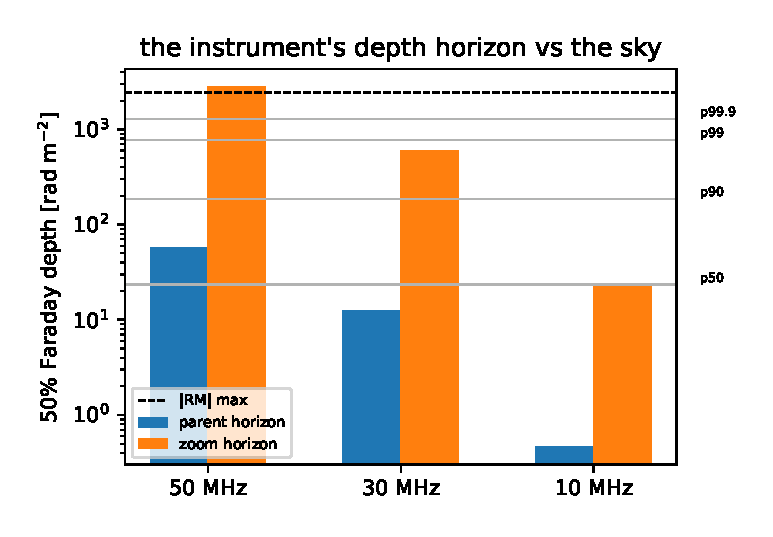
\includegraphics[width=0.62\textwidth]{step5_envelope.pdf}
  \caption{Instrument depth horizons against the beam-weighted sky.
  Horizontal lines are the beam-weighted $|\mathrm{RM}|$ percentiles of
  Table~\ref{tab:horizon}; the dashed line is the map maximum. No parent
  bin reaches the knee; only the 50\,MHz zoom horizon clears the map
  maximum.}
  \label{fig:envelope}
\end{figure}

\subsection{Why a type-3 NUFFT and not an FFT}
\label{sec:chirp}

$\lamsq$ is not uniform in $\nu$. An FFT taken on a uniformly sampled
frequency grid therefore transforms against the wrong conjugate variable,
and a single Faraday depth appears smeared into a chirp whose width grows
with $\phi$. Figure~\ref{fig:chirp} injects one tone at $\phi_0 =
600$\,\rmu{} at 30\,MHz and transforms it both ways.

This matters because the chirp has been misread as a physical limit. It
is not: it is an \emph{analysis artifact}, and it disappears completely
under a type-3 nonuniform transform evaluated on the true \lamsq{} nodes,
which is what Equation~\eqref{eq:rmsynth} is computed with everywhere in
this work. Raw pixel depths can be fed to the same transform as
nonuniform points, and doing so reproduces a direct coherent sum to four
digits.

\begin{figure}[htbp]
  \centering
  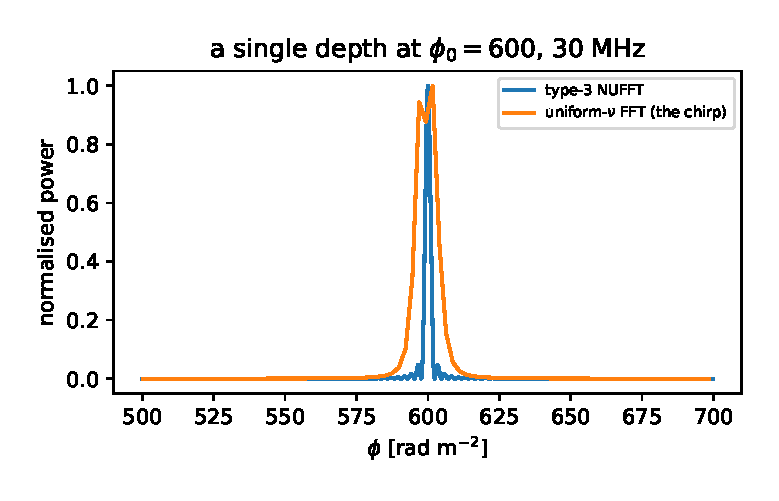
\includegraphics[width=0.62\textwidth]{step5_chirp_coherence.pdf}
  \caption{A single Faraday depth at $\phi_0 = 600$\,\rmu, 30\,MHz,
  transformed on the true \lamsq{} nodes (type-3 NUFFT) and by an FFT on
  a uniform $\nu$ grid. The chirp is an artifact of the second choice.}
  \label{fig:chirp}
\end{figure}

\subsection{Window dynamic range against $\phi\simeq0$ foregrounds}
\label{sec:window}

Instrumental leakage of Stokes $I$ into $Q,U$ is frequency-smooth and
therefore sits at $\phi \simeq 0$. Rejecting it is a question of window
sidelobes, not of the polarimeter. Against a $\phi\simeq0$ foreground at
$|P|/I = 0.15$ through a four-term Blackman--Harris window
\citep{harris1978}, the leakage into depth is $3.7\times10^{-6}$ at the
first sidelobe ($\phi\approx10.8$), $\le 10^{-6}$ beyond $\phi = 27.5$,
$1.4\times10^{-7}$ across the 30\,MHz knee, and $\le 8.8\times10^{-8}$
beyond $\phi = 200$.

The window is therefore \emph{adequate} against both usable ends of the
bracket everywhere the roll-off lives, and inadequate only inside its own
main lobe, $\phi \lesssim 10$. An earlier assessment read the single peak
sidelobe level as a flat floor and concluded the opposite.

\section{The amplitude bracket}
\label{sec:bracket}

The observable amplitude is a fractional polarized amplitude referred to
$T_{\rm sky}$. Three levels are computed, and only their provenance makes
them usable.

\subsection{Incoherent patches (upper)}

If the beam contains $N_{\rm patch}$ polarization patches with
independent angles, their sum is incoherent and the fractional
polarization is suppressed by $N_{\rm patch}^{-1/2}$:
\begin{equation}
  A_{\rm upper} = \frac{1}{\sqrt{N_{\rm patch}}},
  \qquad
  N_{\rm patch} = \frac{\Omega_{\rm beam}}{\theta_c^{2}} .
  \label{eq:upper}
\end{equation}
Here $\Omega_{\rm beam}$ is the effective solid angle of the Faraday
weight, computed as a participation ratio,
$\Omega_{\rm beam} = \bigl(\sum_n |w_n|^2\bigr)^2 / \sum_n |w_n|^4
\times \Omega_{\rm pix}$, and $\theta_c$ is the coherence angle.

$\theta_c$ is defined through the RM structure function
$D(\theta) = \bigl\langle [\phi(\hat n_1) - \phi(\hat n_2)]^2
\bigr\rangle_{|\hat n_1 - \hat n_2| = \theta}$ by
\begin{equation}
  2\,\lambda^{4}\, D(\theta_c) = 1 ,
  \label{eq:thetac}
\end{equation}
i.e. the separation at which the RMS \emph{differential} rotation of the
polarization angle, $2\Delta\phi\lamsq$, reaches $\sqrt2$ radians.
Section~\ref{sec:cannot} shows that Equation~\eqref{eq:thetac} has no
solution this map can resolve, which is why $A_{\rm upper}$ does not
appear in any verdict below.

\subsection{The two power-law floors (lower)}

The floors come from depolarisation \emph{within} the emitting volume.
The distinction that matters is mixed versus external geometry, and it is
the whole question the verdict turns on.

\paragraph{Uniform slab.} For emission distributed uniformly through a
rotating column of total depth $\phi_{\rm col}$ --- the $k=0$ geometry of
Section~\ref{sec:pushforward} --- integrating
Equation~\eqref{eq:rmsynth} over the top-hat gives
\begin{equation}
  \frac{P}{P_0} =
  \left|\int_0^1 e^{2if\phi_{\rm col}\lamsq}\,\mathrm df\right|
  = \left|\frac{\sin(\phi_{\rm col}\lamsq)}{\phi_{\rm col}\lamsq}\right|
  \;\xrightarrow[\ \phi_{\rm col}\lamsq \gg 1\ ]{}\;
  \frac{1}{\phi_{\rm col}\lamsq},
\end{equation}
so, taking the beam-weighted median depth as representative,
\begin{equation}
  A_{\rm slab} = \frac{1}{\bigl|\phi_{\rm med}\bigr|\,\lamsq} .
  \label{eq:slab}
\end{equation}
Note the factor: under the $e^{+2i\phi\lamsq}$ convention the modulus is
$|\sin(\phi\lamsq)/(\phi\lamsq)|$, \emph{not}
$\operatorname{sinc}(2\phi\lamsq)$.

\paragraph{Internal dispersion.} For a mixed medium with turbulent
Faraday dispersion $\sigma$ co-spatial with the emission, Burn's result
\citep{burn1966,sokoloff1998} is
\begin{equation}
  \frac{P}{P_0} = \frac{1 - e^{-2\sigma^{2}\lambda^{4}}}
  {2\sigma^{2}\lambda^{4}}
  \;\xrightarrow[\ 2\sigma^2\lambda^4 \gg 1\ ]{}\;
  \frac{1}{2\sigma^{2}\lambda^{4}},
  \qquad
  A_{\rm disp} = \frac{1}{2\sigma_{\rm eff}^{2}\lambda^{4}},
  \label{eq:disp}
\end{equation}
with $\sigma_{\rm eff} = 9.8$\,\rmu.

\paragraph{Why both floors are power laws.} For an \emph{external}
screen the same dispersion gives Burn's exponential law
$P/P_0 = e^{-2\sigma^2\lambda^4}$. At these wavelengths that is not a
small number, it is zero: at 30\,MHz, $2\sigma^2\lambda^4 \approx
1.9\times10^{6}$. \textbf{A mixed geometry converts exponential
suppression into a power law, and that conversion is the difference
between a detectable signal and no signal at all.} It is also why
Equations~\eqref{eq:slab} and~\eqref{eq:disp} are the two ends of the
usable bracket: they are the two mixed-geometry limits, and which one the
interstellar medium actually sets is not determined here.

Crucially, \textbf{neither floor contains $\theta_c$}. A clamped
coherence angle contaminates $A_{\rm upper}$ alone.

\begin{table}[htbp]
  \centering
  \caption{The amplitude bracket, as fractional polarized amplitude
  referred to $T_{\rm sky}$. $\sigma_{\rm eff} = 9.8$\,\rmu,
  $\phi_{\rm med}$ the beam-weighted median depth.}
  \label{tab:bracket}
  \begin{tabular}{lcccc}
    \toprule
    Level & Formula & 30\,MHz & 50\,MHz & 10\,MHz \\
    \midrule
    $A_{\rm upper}$ & $N_{\rm patch}^{-1/2}$
      & $9.89\times10^{-3}$ & $8.98\times10^{-3}$ & $1.08\times10^{-2}$ \\
    $A_{\rm slab}$ & $1/(|\phi_{\rm med}|\lamsq)$
      & $4.27\times10^{-4}$ & $1.17\times10^{-3}$ & $4.95\times10^{-5}$ \\
    $A_{\rm disp}$ & $1/(2\sigma_{\rm eff}^2\lambda^4)$
      & $5.22\times10^{-7}$ & $4.03\times10^{-6}$ & $6.45\times10^{-9}$ \\
    \midrule
    \multicolumn{5}{l}{\emph{$A_{\rm upper}$ is not computable from this
    map (\S\ref{sec:cannot}) and is excluded from every verdict.}}\\
    \bottomrule
  \end{tabular}
\end{table}

\subsection{The coherence tilt is a shape systematic}

Equation~\eqref{eq:identity} holds exactly only when the patch coherence
scale is independent of depth. It is not: nearby low-$\phi$ emission
subtends larger coherent patches than distant high-$\phi$ emission. Per
depth cell, coherent patches add as $N_{\rm patch}^2$ against
$N_{\rm patch}$ incoherent, so a depth-dependent patch count \emph{tilts
the shape} --- boosting the low-$\phi$ core relative to the tail, most
strongly at the roll-off where the beam contains fewest patches. This is
carried as a second bracket, drawn as the dotted companion curves in
Figure~\ref{fig:family}, and it is a systematic on the shape, not on the
normalisation.

\section{Noise and the matched filter}
\label{sec:noise}

\subsection{Radiometer noise into zoom bins}

Per bin of width $\Delta\nu$ and integration $\Delta t$,
\begin{equation}
  \sigma = \frac{T_{\rm sys}}{\sqrt{\Delta\nu\,\Delta t}} .
  \label{eq:radiometer}
\end{equation}
The zoom bins are \emph{not} independent. Their equivalent noise
bandwidth is $563$\,Hz on a $390.625$\,Hz spacing --- a $1.44\times$
overlap --- so white noise on the fine channels produces a correlated bin
covariance. With $W$ the column-normalised fine-to-bin weight matrix,
\begin{equation}
  N_{ij} = \sigma^{2}\,\frac{G_{ij}}{\sqrt{G_{ii}\,G_{jj}}},
  \qquad G = W^{\!\top}W ,
  \label{eq:noisecov}
\end{equation}
which has unit diagonal by construction and a measured
nearest-neighbour correlation of $0.15$ --- of order the real overlap,
not zero.

\subsection{The whitened matched filter}

Model the Faraday signal as a Gaussian random field of known normalised
shape $\hat H$ and unknown amplitude $A$. Its frequency covariance is
\begin{equation}
  S_{ij} = \sum_b \hat H_b\,
  e^{2i\phi_b(\lamsq_i - \lamsq_j)},
  \qquad \sum_b \hat H_b = 1 ,
  \label{eq:sigcov}
\end{equation}
so $\operatorname{diag} S = 1$ and amplitude $A$ means per-bin signal
power $A^2$. For a Gaussian-signal likelihood ratio with $M$ independent
LST samples and $n$ coherent nights, the Fisher information gives
\begin{equation}
  \mathrm{SNR} = n\,A^{2}\sqrt{M\,
  \operatorname{tr}\!\bigl[(N^{-1}S)^2\bigr]},
  \qquad
  A_{5\sigma} = \sqrt{\frac{5}{n\sqrt{M\,
  \operatorname{tr}[(N^{-1}S)^2]}}} .
  \label{eq:mf}
\end{equation}
Equation~\eqref{eq:mf} carries the covariance of
Equation~\eqref{eq:noisecov} rather than assuming independent modes.
Holding everything else fixed and replacing $N$ by its diagonal degrades
the threshold by a measured factor $\mathbf{1.160}$: that ratio, not any
comparison to a closed form, is the cost of the overlap.

A closed form is carried as a sanity check with different assumptions ---
noise per coherence cell and independent modes:
\begin{equation}
  A_{\rm closed} = \sigma_{\rm mode}
  \sqrt{\frac{5}{n\sqrt{N_{\rm modes}}}},
  \qquad
  \sigma_{\rm mode} = \frac{1}{\sqrt{\Delta\nu_{\rm coh}\,\tau}} .
  \label{eq:closed}
\end{equation}
At 24 lunations the two agree to $2\%$ at 30\,MHz
($1.328\times10^{-5}$ against $1.354\times10^{-5}$) and diverge at the
other two bands --- the matched filter is $16\%$ worse at 50\,MHz and
$46\%$ better at 10\,MHz --- because the closed form's fixed coherence
bandwidth is a poor description of the real signal covariance there.
Equation~\eqref{eq:mf} is the deliverable; Equation~\eqref{eq:closed} is
a check on it, not a bound.

\section{Results}
\label{sec:results}

\subsection{The template family}

Figure~\ref{fig:family} is the deliverable: a normalised shape per band,
per geometry, with the coherence bracket as its companion. All numbers in
this section are for the fiducial $k=0$ uniform slab and the as-built
four-port arm unless stated.

\begin{figure}[htbp]
  \centering
  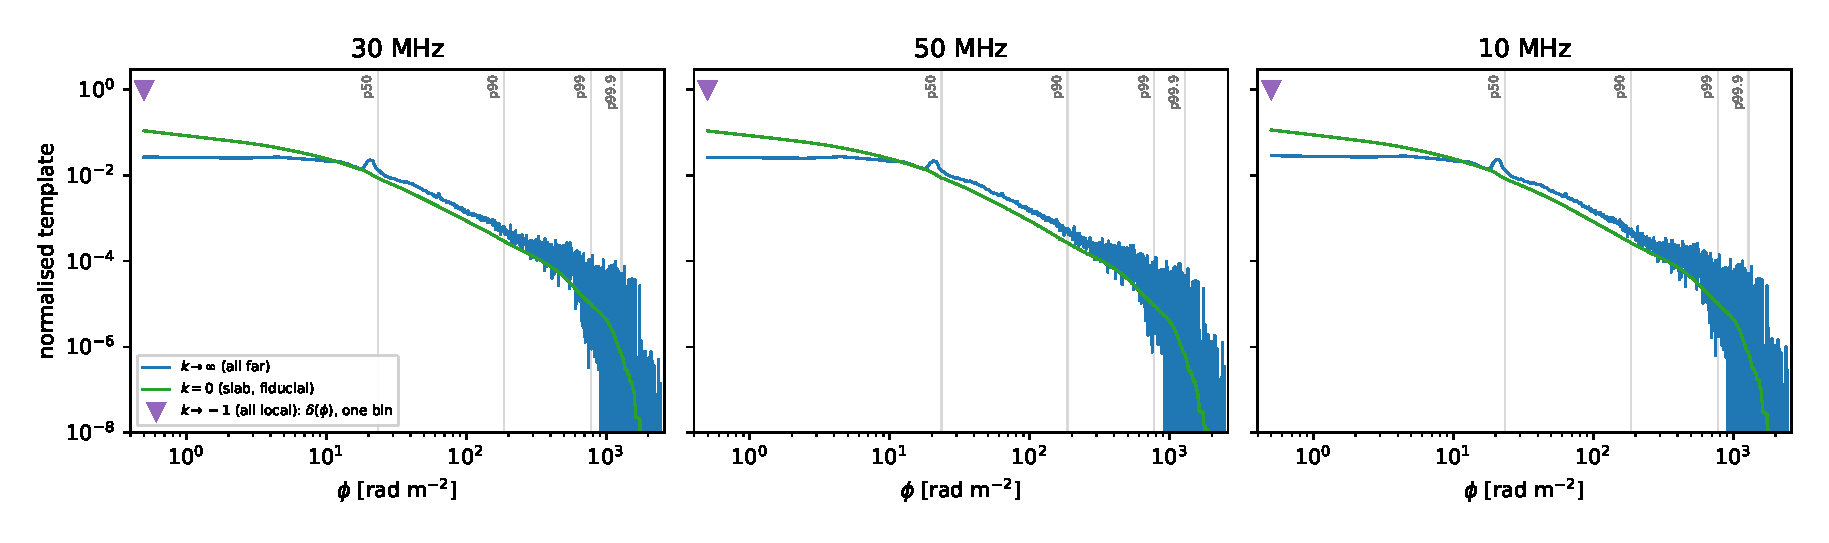
\includegraphics[width=\textwidth]{step5_template_family.pdf}
  \caption{The normalised delay-space template for the three bands and
  the three emissivity geometries of Section~\ref{sec:pushforward}.
  Solid: the incoherent template. Dotted: the coherence-tilted companion.
  Grey verticals: the beam-weighted $|\mathrm{RM}|$ percentiles of
  Table~\ref{tab:horizon}.}
  \label{fig:family}
\end{figure}

The roll-off statistic is the \textbf{90\%-mass quantile} of the folded
template --- a CDF quantile, not a half-power crossing. The distinction
is not cosmetic: a half-power statistic pins to the narrow spike the
$k=0$ slab piles up at the origin, which is why an earlier half-power
version was measured to be defective and replaced.

\subsection{Robustness of the shape}
\label{sec:robust}

\begin{table}[htbp]
  \centering
  \caption{The 90\%-mass knee at $k=0$ under two perturbations. Units
  \rmu.}
  \label{tab:robust}
  \begin{tabular}{lccccc}
    \toprule
    Band & knee & plane-tapered & taper factor & two-port arm & arm swap \\
    \midrule
    30\,MHz & 89.62 & 17.95 & $4.99\times$ & 88.99  & $-0.7\%$ \\
    50\,MHz & 83.32 & 19.26 & $4.33\times$ & 102.99 & $+23.6\%$ \\
    10\,MHz & 83.91 & 18.03 & $4.66\times$ & 94.09  & $+12.1\%$ \\
    \bottomrule
  \end{tabular}
\end{table}

\paragraph{Plane taper.} Down-weighting the Galactic plane by
$\sin^2|b|$ moves the knee by a factor $4.3$--$5.0$, so
\textbf{the roll-off is carried by the plane}, not by high-$|b|$
sightlines. This is the \emph{unfavourable} branch. Long in-plane paths
are exactly where the line-of-sight field $B_\parallel$ reverses and the
linear $\phi(f)$ ansatz of Section~\ref{sec:pushforward} is weakest, so
the geometry assumption is doing real work and \textbf{the amplitude
bracket must be read as wider, not narrower}, than
Table~\ref{tab:bracket} suggests. The \emph{direction} of the reversal
effect is favourable --- reversals broaden $F$ outward, so the computed
roll-off is a lower bound on the extent --- but its size is not bounded
by anything computed here.

\paragraph{Two arms.} Swapping the as-built four-port $|w|^2$ for the
symmetric two-port pseudo-dipole moves the knee by $+23.6\%$ at 50\,MHz
and $+12.1\%$ at 10\,MHz, but by $-0.7\%$ at 30\,MHz. The two beams
weight different declination strips and therefore see different parts of
the RM sky; at the band that owns the knee, they agree.
Figure~\ref{fig:twoarm} shows the full templates.

\begin{figure}[htbp]
  \centering
  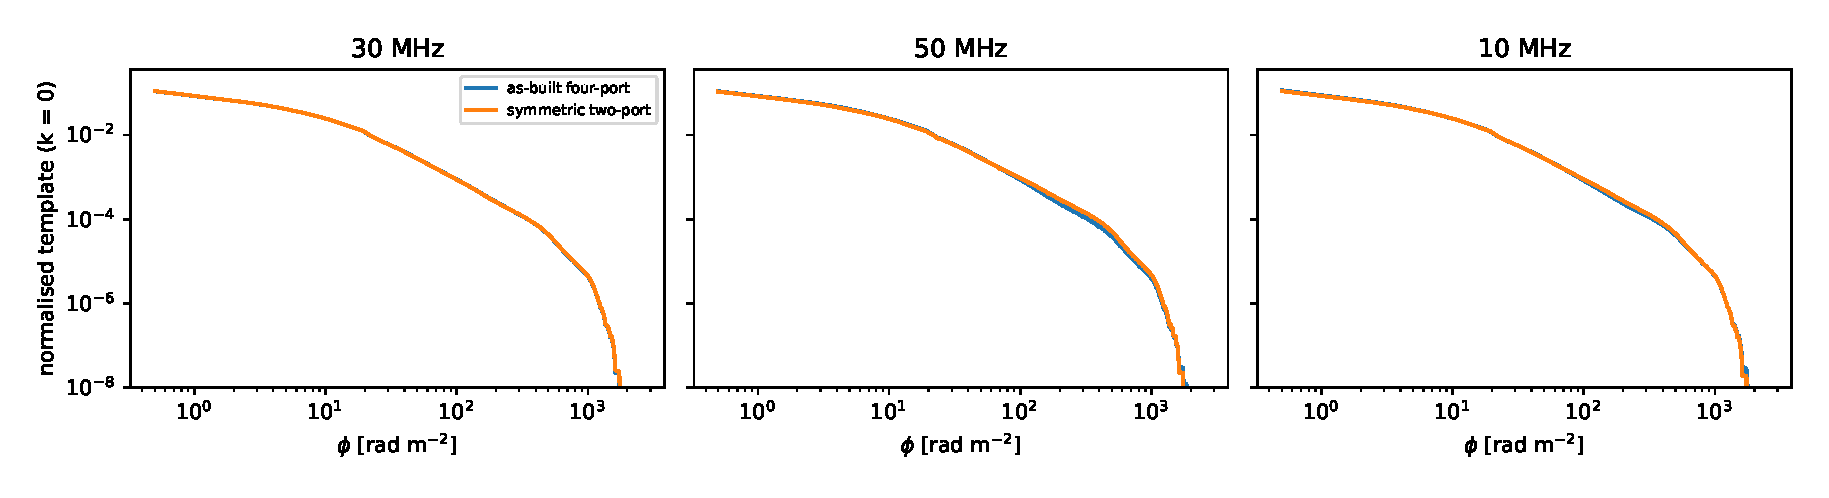
\includegraphics[width=\textwidth]{step5_two_arm.pdf}
  \caption{The $k=0$ template through the as-built four-port response and
  through the symmetric two-port pseudo-dipole. The beam enters only
  through $|w|^2$, so this is a single input substitution.}
  \label{fig:twoarm}
\end{figure}

\subsection{The tail, resolved over sidereal time}

Localising the signal in depth --- as opposed to detecting it --- depends
on template power \emph{above} the bulk of the sky's depth distribution.
Define the tail fraction as the fraction of template power above the
fixed beam-weighted p99 threshold. Figure~\ref{fig:knee} resolves it over
a full lunation.

\begin{figure}[htbp]
  \centering
  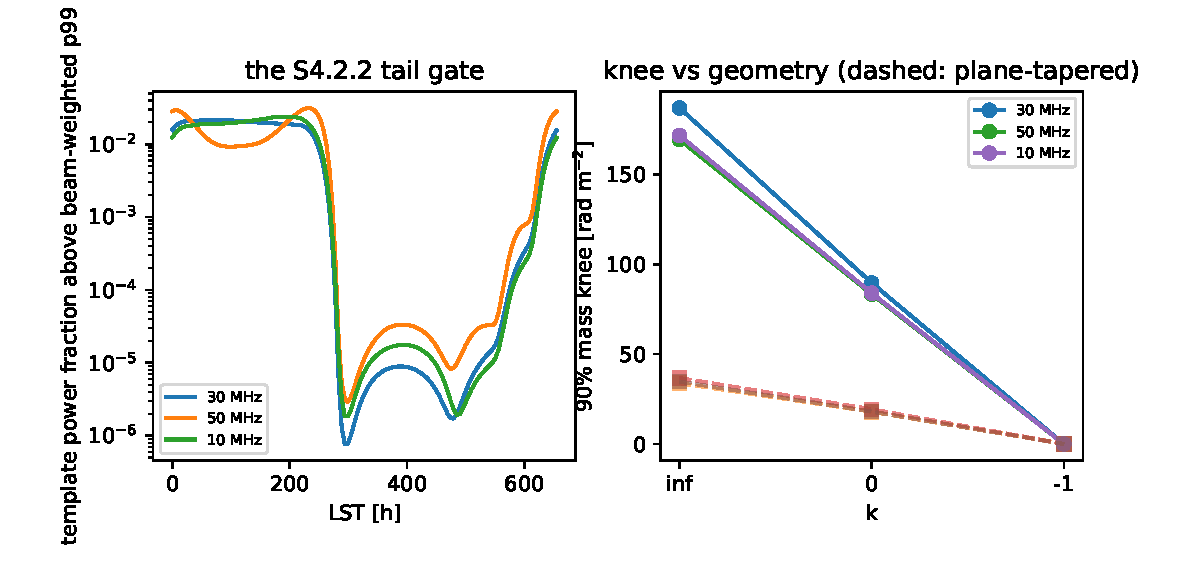
\includegraphics[width=\textwidth]{step5_knee_tail_lst.pdf}
  \caption{Left: the tail fraction over local sidereal time, peaking
  sharply at Galactic Centre transit. Right: the 90\%-mass knee per band
  against the emissivity geometry, with the plane-tapered version
  overlaid (dashed).}
  \label{fig:knee}
\end{figure}

\begin{table}[htbp]
  \centering
  \caption{The tail fraction $f$: fraction of template \emph{power}
  above the fixed beam-weighted p99 threshold.}
  \label{tab:tail}
  \begin{tabular}{lccc}
    \toprule
    Band & GC-transit maximum & LST mean & two-port arm, transit \\
    \midrule
    30\,MHz & 2.16\% & 0.81\% & 2.18\% \\
    50\,MHz & 3.15\% & 0.81\% & 3.70\% \\
    10\,MHz & 2.39\% & 0.82\% & 2.69\% \\
    \bottomrule
  \end{tabular}
\end{table}

Away from transit the fraction falls to $\sim10^{-6}$. The LST mean sits
near $0.8\%$ at every band and arm --- close to the $\sim1\%$ the p99
definition implies at a typical LST --- and Galactic Centre transit lifts
it only $2$--$4\times$ above that floor, not by orders of magnitude. The
measurement is solid: the two arms agree to within $0.6$ percentage
points at every band.

\section{The verdict}
\label{sec:verdict}

\subsection{The convention that moves every number}

$f$ in Table~\ref{tab:tail} is a fraction of the template's
\emph{power}; the bracket in Table~\ref{tab:bracket} is an
\emph{amplitude}. Detection and localisation are separated by roughly the
square root of the tail's power fraction, so the tail's amplitude is
\begin{equation}
  A_{\rm tail} = A_{\rm bracket} \times \sqrt{f},
  \qquad\text{not}\qquad A_{\rm bracket}\times f .
  \label{eq:sqrtf}
\end{equation}
At 30\,MHz, $\sqrt{0.0216} = 0.147$ against $f = 0.0216$: a factor
$6.8$ on every ratio below. An earlier version of this arithmetic lost
it.

\subsection{The gate}

\begin{table}[htbp]
  \centering
  \caption{The tail gate. $A_{\rm mf}$ is the $5\sigma$ whitened
  matched-filter threshold of Equation~\eqref{eq:mf} at 24 lunations;
  tail amplitudes are Equation~\eqref{eq:sqrtf}. $A_{\rm upper}$ is
  excluded --- see \S\ref{sec:cannot}.}
  \label{tab:verdict}
  \begin{tabular}{lcc cc cc}
    \toprule
    & & & \multicolumn{2}{c}{at $A_{\rm slab}$}
      & \multicolumn{2}{c}{at $A_{\rm disp}$} \\
    \cmidrule(lr){4-5}\cmidrule(lr){6-7}
    Band & $A_{\rm mf}$ & $f$ & $A_{\rm tail}$ & ratio
      & $A_{\rm tail}$ & ratio \\
    \midrule
    30\,MHz & $1.33\times10^{-5}$ & 2.16\%
      & $6.26\times10^{-5}$ & \textbf{4.72 OPEN}
      & $7.66\times10^{-8}$ & 0.006 closed \\
    50\,MHz & $1.07\times10^{-5}$ & 3.15\%
      & $2.07\times10^{-4}$ & \textbf{19.35 OPEN}
      & $7.15\times10^{-7}$ & 0.067 closed \\
    10\,MHz & $1.67\times10^{-5}$ & 2.39\%
      & $7.65\times10^{-6}$ & 0.458 closed
      & $9.96\times10^{-10}$ & $6.0\times10^{-5}$ closed \\
    \bottomrule
  \end{tabular}
\end{table}

\textbf{The gate opens at 30 and 50\,MHz if the diffuse amplitude sits at
the uniform-slab floor, and closes at every band if it sits at the
internal-dispersion floor.} By Section~\ref{sec:bracket} that is a
mixed-versus-external-screen geometry question about the interstellar
medium, and it is the single unknown the science case turns on.

Taking the two-port arm consistently --- its own bracket against its own
$\sqrt f$, never a mixture --- gives $4.77 / 19.92 / 0.466$, at most
$3\%$ away, with the same OPEN/closed calls at every band. The verdict is
not an artifact of which instrument arm weights the sky.

\subsection{What does not decide it}

\paragraph{Not the tail measurement.} $f$ is solid at $2.2$--$3.7\%$
across both arms (Table~\ref{tab:tail}). Even an order-of-magnitude error
in $f$ moves the ratios by only $\sqrt{10} = 3.2$.

\paragraph{Not $\theta_c$.} Both floors in Table~\ref{tab:verdict} are
$\theta_c$-free by Equations~\eqref{eq:slab} and~\eqref{eq:disp}. Only
$A_{\rm upper}$ contains it, and $A_{\rm upper}$ is excluded.

\paragraph{Not integration time.} Adding nights scales the threshold as
$n^{-1/2}$. At 30\,MHz the internal-dispersion floor sits $173\times$
below threshold, so closing that gap by integrating alone would take
$173^2 \approx 3\times10^{4}$ times more nights. Integration is not the
lever.

Figure~\ref{fig:sensitivity} draws the threshold curve against the
bracket. Note the caption on the figure itself: the dashed upper line
alone derives from $\theta_c$ and is a clamp-derived bound, not a
measurement.

\begin{figure}[htbp]
  \centering
  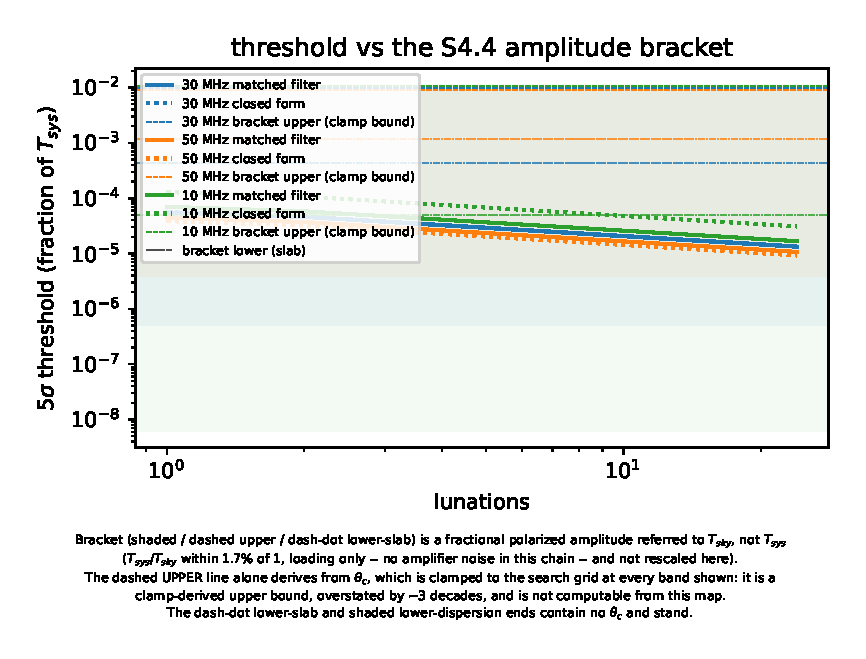
\includegraphics[width=0.78\textwidth]{step5_sensitivity.pdf}
  \caption{The $5\sigma$ whitened matched-filter threshold against
  lunations, with the closed form of Equation~\eqref{eq:closed} dotted,
  and the amplitude bracket of Table~\ref{tab:bracket} shaded. The
  threshold curves are fractions of $T_{\rm sys}$ and the bracket is
  referred to $T_{\rm sky}$; the two reference temperatures differ by
  $\le1.7\%$ (\S\ref{sec:cannot}) and nothing is rescaled.}
  \label{fig:sensitivity}
\end{figure}

\section{What this map cannot decide}
\label{sec:cannot}

Both items below are limitations of the inputs, not of the method. They
are stated here rather than in a footnote because a reader who takes
Table~\ref{tab:bracket}'s first row or the ratio $T_{\rm sys}/T_{\rm
sky}$ at face value will draw a wrong conclusion.

\subsection{The bracket's upper end is not computable}
\label{sec:clamp}

Equation~\eqref{eq:thetac} is solved by inverting a Monte-Carlo estimate
of $D(\theta)$ on a grid spanning $0.2^\circ$ to $30^\circ$. At every
band and in both arms the solution \textbf{clamps at the grid's lower
edge}.

The clamp \emph{overstates}. Because $D$ is monotonised before
inversion, a target below $D(\theta_{\min})$ means the root lies below
the grid, and returning $\theta_{\min}$ returns something larger than the
root --- so a clamped $\theta_c$ is an upper bound, and
$A_{\rm upper} \propto \theta_c$ inherits that. The size of the
overstatement is measurable on the script's own grid:
$D(0.2^\circ) = 96.2\,(\rmu)^2$ against targets $5.01\times10^{-5}$,
$3.87\times10^{-4}$ and $6.19\times10^{-7}$ at $30/50/10$\,MHz, i.e. a
root $1385\times$, $499\times$ and $12\,465\times$ below the grid edge
under $D \propto \theta^2$.

\textbf{Widening the grid cannot fix it.} Extrapolating $D\propto\theta^2$
puts the root at $0.52''$, $1.44''$ and $0.058''$ --- two and a half to
nearly four decades below the $412''$ pixel scale of the nside-512
Faraday map itself. A wider search grid would \emph{extrapolate} the
structure function, not measure it. The internal evidence that the
extrapolation is not quotable is that it inverts the bracket: at 30\,MHz
it gives $A_{\rm upper} = 7.1\times10^{-6}$, which is \emph{below}
$A_{\rm slab} = 4.27\times10^{-4}$.

\textbf{The incoherent-patch upper bound is not determinable from this
map} and must be quoted as such, never as $\sim\!10^{-2}$. The two lower
levels contain no $\theta_c$ and stand.

\subsection{Sky domination at 50\,MHz is open}

The computed ratio is
$T_{\rm sys}/T_{\rm sky} = 1.0044 / 1.0170 / 1.0006$ at
$30/50/10$\,MHz. Read it as $1 + T_{\rm loading}/T_{\rm sky}$ and
nothing more: the modelled signal chain carries \textbf{no amplifier
noise}, so the term this check exists to bound --- receiver noise through
a short, mismatched dipole on regolith at 50\,MHz --- is set to zero.
Furthermore $T_{\rm sky}$ here is an all-sky mean of Stokes $I$ rather
than a beam-weighted antenna temperature.

It is therefore a genuine \emph{lower bound}, not a computed
sky-domination result. What it does establish is that moon and loss
loading is a $\le1.7\%$ correction, so the reference-temperature mismatch
in Figure~\ref{fig:sensitivity} is quantitatively negligible.
\textbf{Sky domination at 50\,MHz remains open} until a receiver noise
temperature is supplied.

\subsection{Two limits already stated}

For completeness, the two limits of Section~\ref{sec:identity} belong on
this list: the acceptance gates do not test the incoherent-limit
identity, and the identity does not demonstrate that the sky is
incoherent.

\section{Reproducing this}
\label{sec:repro}

Every number in this report comes from committed code. The heavy
products are regenerable but not tracked (25\,MB each); the six figures
are tracked so this document builds from a fresh checkout.

\subsection{Products and scripts}

\begin{center}
\begin{tabular}{lll}
\toprule
Product & Script & Contains \\
\midrule
\code{step5\_envelope.npz} & \code{step5\_instrument\_envelope.py}
  & Table~\ref{tab:horizon} \\
\code{step5\_template.npz} & \code{step5\_template.py --lst 128}
  & Tables~\ref{tab:bracket},~\ref{tab:robust},~\ref{tab:tail} \\
\code{step5\_template\_two\_port.npz} & \code{... --arm two-port}
  & arm columns \\
\code{step5\_sensitivity.npz} & \code{step5\_sensitivity.py}
  & Table~\ref{tab:verdict} \\
figures & \code{step5\_plots.py}
  & Figures~\ref{fig:envelope}--\ref{fig:sensitivity} \\
\bottomrule
\end{tabular}
\end{center}

Table~\ref{tab:rmsf} is computed live, in about two seconds, and needs
no data products at all. A companion notebook,
\code{notebooks/faraday\_delay\_template.ipynb}, is committed
\emph{executed} and reproduces Tables~\ref{tab:rmsf},
\ref{tab:robust}--\ref{tab:verdict} and every figure here from the
products above.

\subsection{Which test pins which claim}

\begin{center}
\footnotesize
\begin{tabular}{ll}
\toprule
Claim & Test \\
\midrule
Shape stable under refinement
  & \code{test\_gate1\_shape\_invariance\_under\_refinement} \\
Shape stable under null rotation
  & \code{test\_gate2\_shape\_invariance\_under\_null\_rotation} \\
The identity, Eq.~\eqref{eq:identity}
  & \code{test\_delay\_power\_equals\_the\_weighted\_depth\_distribution} \\
Converged control through the NUFFT
  & \code{test\_converged\_regime\_points\_match\_direct\_sum} \\
Depth horizons, Table~\ref{tab:horizon}
  & \code{test\_depth\_horizon\_pins\_the\_s46\_table} \\
Resolution and convention, Table~\ref{tab:rmsf}
  & \code{test\_boxcar\_rmsf\_widths} \\
NUFFT beats FFT, \S\ref{sec:chirp}
  & \code{test\_nufft\_beats\_fft\_on\_a\_single\_depth} \\
Window budget, \S\ref{sec:window}
  & \code{test\_foreground\_sidelobe\_budget} \\
$\theta_c$ clamps below the grid, \S\ref{sec:clamp}
  & \code{test\_coherence\_angle\_clamps\_below\_the\_sampled\_range} \\
Bracket closed forms, Eqs.~\eqref{eq:slab},~\eqref{eq:disp}
  & \code{test\_amplitude\_bracket\_closed\_forms} \\
Overlap degradation $1.160\times$
  & \code{test\_overlap\_correlation\_degrades\_the\_threshold} \\
Matched filter, Eq.~\eqref{eq:mf}
  & \code{test\_matched\_filter\_monte\_carlo} \\
Tail-gate arithmetic, \S\ref{sec:verdict}
  & \code{test\_tail\_gate\_extraction\_is\_numerically\_inert} \\
\bottomrule
\end{tabular}
\end{center}

\subsection{Building this document}

\begin{verbatim}
    cd report/delay_template && make
\end{verbatim}

\section*{Acknowledgements}

This work uses the Galactic Faraday rotation sky of
\citet{hutschenreuter2022}, the destriped 408\,MHz map of
\citet{remazeilles2015}, the nine-year WMAP polarization maps of
\citet{bennett2013}, the HEALPix pixelisation \citep{gorski2005}, and
the FINUFFT library \citep{barnett2019}.

\begin{thebibliography}{99}

\bibitem[Barnett et al.(2019)]{barnett2019}
Barnett, A.~H., Magland, J., \& af Klinteberg, L. 2019,
\emph{A Parallel Nonuniform Fast Fourier Transform Library Based on an
``Exponential of Semicircle'' Kernel},
SIAM Journal on Scientific Computing, 41, C479

\bibitem[Bennett et al.(2013)]{bennett2013}
Bennett, C.~L., Larson, D., Weiland, J.~L., et al. 2013,
\emph{Nine-year Wilkinson Microwave Anisotropy Probe (WMAP)
Observations: Final Maps and Results},
ApJS, 208, 20

\bibitem[Brentjens \& de Bruyn(2005)]{brentjens2005}
Brentjens, M.~A., \& de Bruyn, A.~G. 2005,
\emph{Faraday rotation measure synthesis},
A\&A, 441, 1217

\bibitem[Burn(1966)]{burn1966}
Burn, B.~J. 1966,
\emph{On the depolarization of discrete radio sources by Faraday
dispersion},
MNRAS, 133, 67

\bibitem[G\'orski et al.(2005)]{gorski2005}
G\'orski, K.~M., Hivon, E., Banday, A.~J., et al. 2005,
\emph{HEALPix: A Framework for High-Resolution Discretization and Fast
Analysis of Data Distributed on the Sphere},
ApJ, 622, 759

\bibitem[Harris(1978)]{harris1978}
Harris, F.~J. 1978,
\emph{On the use of windows for harmonic analysis with the discrete
Fourier transform},
Proceedings of the IEEE, 66, 51

\bibitem[Hutschenreuter et al.(2022)]{hutschenreuter2022}
Hutschenreuter, S., Anderson, C.~S., Betti, S., et al. 2022,
\emph{The Galactic Faraday rotation sky 2020},
A\&A, 657, A43

\bibitem[Remazeilles et al.(2015)]{remazeilles2015}
Remazeilles, M., Dickinson, C., Banday, A.~J., Bigot-Sazy, M.-A., \&
Ghosh, T. 2015,
\emph{An improved source-subtracted and destriped 408-MHz all-sky map},
MNRAS, 451, 4311

\bibitem[Sokoloff et al.(1998)]{sokoloff1998}
Sokoloff, D.~D., Bykov, A.~A., Shukurov, A., et al. 1998,
\emph{Depolarization and Faraday effects in galaxies},
MNRAS, 299, 189

\end{thebibliography}

\end{document}
